\section{Цель работы}
Ознакомление с основными приемами работы с документацией при
составлении программ для микроконтроллеров. Приобретение навыков работы с
осциллографом и оценочной платой MCBSTM32F200 в качестве измерительного
генератора	.

\section{Постановка задачи}
Используя библиотеки Keil µVision5, разработать
программу для микроконтроллера (МК) STM32F200, которая включает и выключает
светодиод.
\section{Алгоритм работы программы}

Данный раздел описывает последовательность действий, необходимых для разработки и реализации проекта на базе микроконтроллера STM32F207IGHx в среде Keil~µVision5. Алгоритм включает этапы инициализации проекта, настройки портов ввода–вывода, реализации мигания светодиода и модификации программы для создания эффекта «бегущего огня».

\subsection{Инициализация проекта}
\begin{itemize}
    \item Создание нового проекта в среде Keil \(\mu\)Vision5.
    \item Выбор микроконтроллера \textbf{STM32F207IGHx}.
    \item Настройка параметров проекта, включая поддержку ядра (\textit{CMSIS CORE}), запуск (\textit{Startup}) и настройки HAL.
    \item Подключение библиотеки \texttt{stm32f2xx.h}, где хранится информация обо всех адресах регистров.
\end{itemize}

\subsection{Настройка порта GPIOG}
\begin{itemize}
    \item Включение тактирования порта GPIOG через регистр \texttt{RCC\_AHB1ENR}.
    \item Переключение режима работы GPIOG в режим вывода через регистр \texttt{GPIOG\_MODER}.
\end{itemize}

\subsection{Используемые переменные и регистры}
\begin{description}
    \item \texttt{RCC->AHB1ENR} — включает тактирование периферийных устройств, используется для активации GPIOG.
    \item \texttt{GPIOG->MODER} — задает режим работы пина PG7 (настроен как выход).
    \item \texttt{GPIOG->ODR} — управляет включением и выключением светодиода.
\end{description}

\subsection{Реализация мигания светодиода}
\begin{enumerate}
    \item Установка бита PG7 в \texttt{GPIOG\_ODR} в "1" (включение светодиода).
    \item Ожидание задержки для визуального восприятия мигания.
    \item Сброс бита PG7 в \texttt{GPIOG\_ODR} в "0" (выключение светодиода).
    \item Повторение цикла для непрерывного мигания.
\end{enumerate}

\section{Ответ на вопросы до работы с осциллографом}
\begin{enumerate}
	\item A: 8x10 делений
	\item B: 5V
	\item C: Масштаб станет равным 5В/деление, а сигнал будет занимать 2 вертикальных деления
	\item A: 500 µS
	\item B: 1250 Hz
\end{enumerate}

\section{Полученные результаты}
\begin{itemize}
	\item Успешно создан проект в Keil μVision5.
	\item Разработана программа, которая управляет светодиодом на оценочной плате MCBSTM32F200.
	\item Программа корректно работает: светодиод мигает с заданной частотой.
	\item Модифицированная программа с бегущей строкой также успешно протестирована.
\end{itemize}




\newpage

\section*{Код программы}

\begin{lstlisting}[style=cstyle, caption={Основная функция программы}]
#include "stm32f2xx.h" // Подключаем библиотеку, где лежат адреса всех регистров

// Функция реализации задержки
void delay ()
{
    unsigned long i; // Переменная для счетчика цикла
		// Цикл, который просто выполняется много раз, чтобы создать задержку
    for(i=0; i<2000000; i++){} 
}



// Главная функция программы
int main ()
{
    // 1. Включение тактирования порта G (через регистр RCC_AHB1ENR)
    // Чтобы порт заработал, на него надо подать тактовую частоту.
    // За порт G отвечает 6-й бит в этом регистре.
    // Нам нужно записать туда единицу.
    // Считаем значение: 1 сдвигаем влево на 6 раз.
    // Это 2 в степени 6 = 64. В 16-ричной системе это 0x40.
    RCC->AHB1ENR |= 1ul<<6; 

    // 2. Настройка пина 7 на выход (через регистр GPIOG_MODER)
    // В этом регистре на каждый пин дается по 2 бита настроек.
    // Номер пина 7. Значит его биты это 14 и 15 (7 * 2 = 14).
    // Чтобы пин стал выходом (Output), нужно записать код 01.
    // То есть: в 15-й бит записать 0, а в 14-й бит записать 1.
    
    // Сначала сбрасываем 15-й бит в ноль.
    // 2 в степени 15 = 32768 (или 0x8000). Используем значок ~ чтобы сделать инверсию.
    
    // Потом устанавливаем 14-й бит в единицу.
    // 2 в степени 14 = 16384 (или 0x4000).
    
    // Объединяем эти действия в одной строке:
    GPIOG->MODER = (GPIOG->MODER & ~1ul<<15) | 1ul<<14;

    // Бесконечный цикл, чтобы программа не заканчивалась
    for (;;)
    {
        // 3. Включаем светодиод (через регистр GPIOG_ODR)
        // Чтобы зажечь диод на пине 7, нужно в 7-й бит записать 1.
        // Считаем: 2 в степени 7 = 128. В 16-ричной системе это 0x80.
        // Операция |= ставит бит в 1.
        GPIOG->ODR |= 1ul<<7;

        delay (); // Ждем, чтобы увидеть свет

        // 4. Выключаем светодиод
        // Чтобы погасить диод на пине 7, нужно в 7-й бит записать 0.
        // Используем то же число (2 в степени 7 = 128).
        // Но используем операцию &= ~ (И с инверсией), чтобы сбросить бит в 0.
        GPIOG->ODR &= ~1ul<<7;

        delay (); // Ждем в выключенном состоянии
    }
}
\end{lstlisting}

\section{Работа с осциллографом}
Для измерения был получен снимок нескольких тактов сигнала:
\begin{itemize}
	\item Размах сигнала: 3.2 В
	\item Период сигнала: 1.5 с
	\item Частота сигнала: 0.66 Гц
	\item Ширина положительного уровня: 0.75 с
	\item Ширина отрицательного уровня: 0.75 с
	\item Коэффициент заполнения: 0.5
\end{itemize}
\newpage


\begin{figure}[h!]
\centering
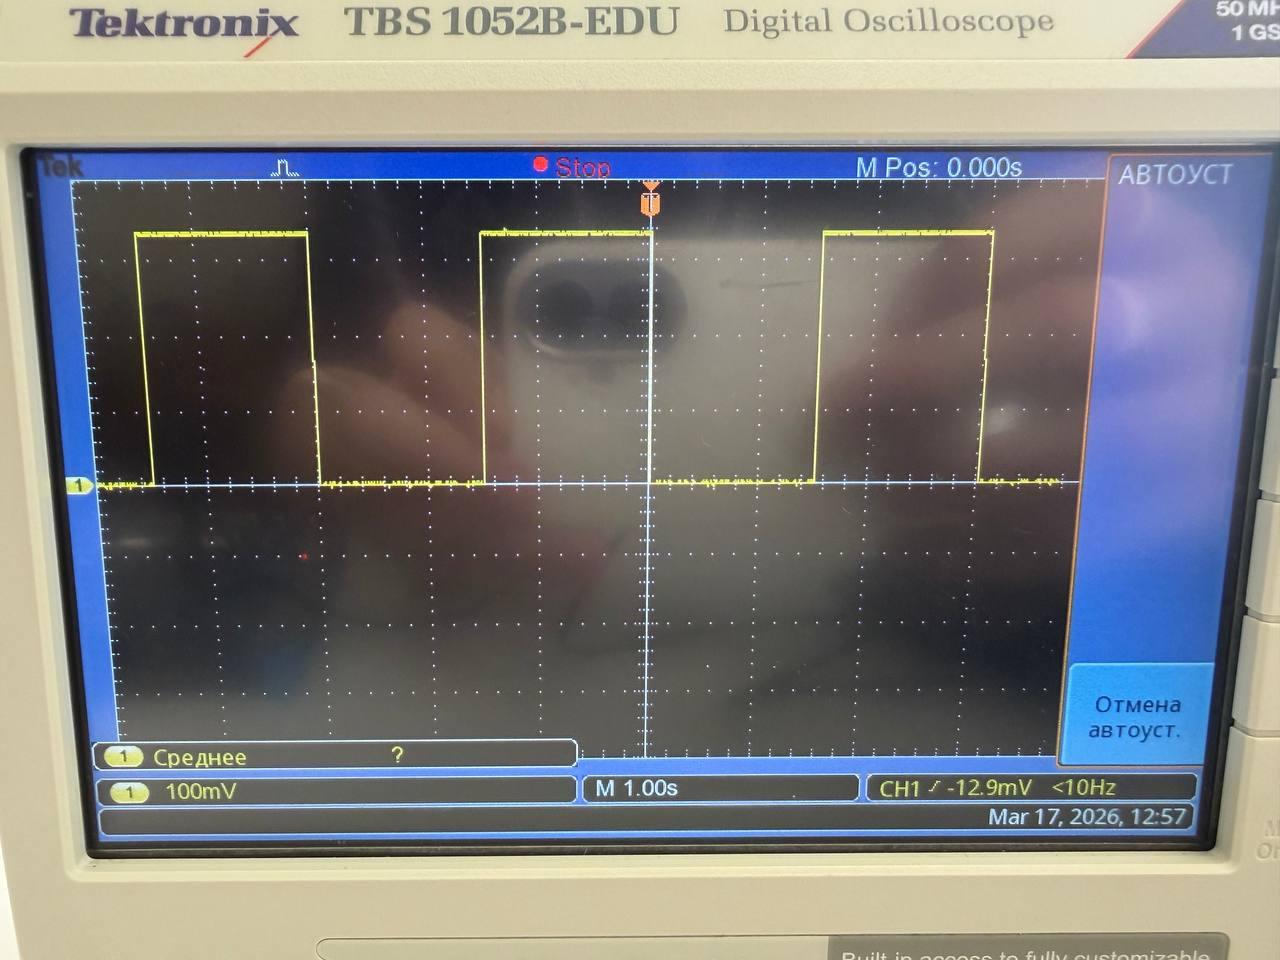
\includegraphics[width=0.9\textwidth]{Photo/1.jpg}
\end{figure}
Для измерения времени нарастания формы волны был получен другой
снимок.
Время нарастания от 20\% сигнала до 80\%: 6.5 нс

\begin{figure}[h!]
\centering

\includegraphics[width=0.9\textwidth]{Photo/2.jpg}
\end{figure}
Для измерения времени затухания формы волны был получен другой снимок.
Время затухания от 20\% сигнала до 80\%: 6.5 нс

\begin{figure}[h!]
\centering

\includegraphics[width=0.9\textwidth]{Photo/3.jpg}
\end{figure}

Далее нужно было изменить задержки в программе так, чтобы значение
скважности стало 1/3. Для этого нужно было задержку после включения
светодиода увеличить в 2 раза.

\begin{figure}[h!]
\centering
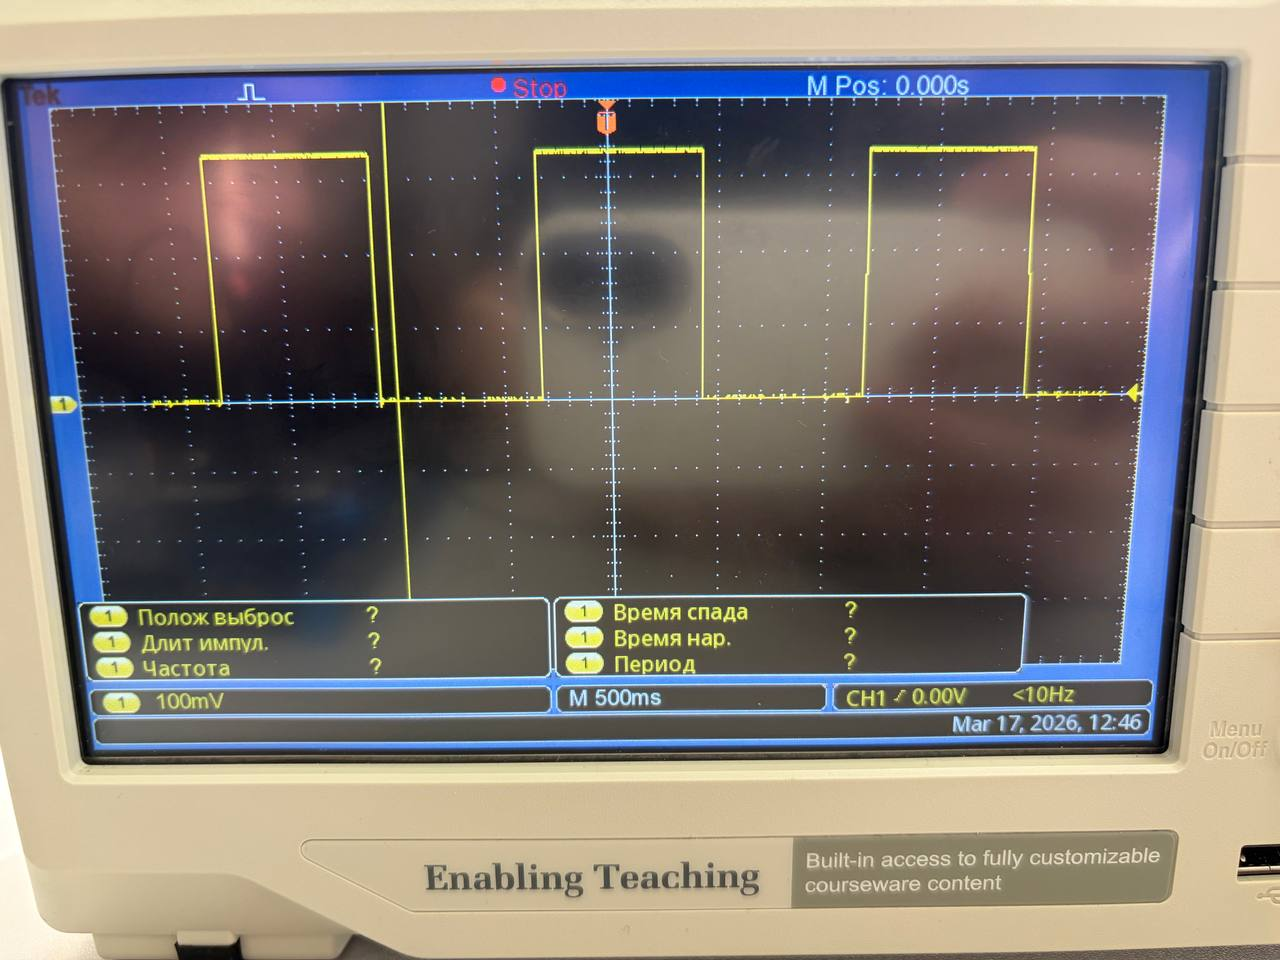
\includegraphics[width=0.9\textwidth]{Photo/4.jpg}
\end{figure}

\newpage

\section{Результаты работы с осциллографом}

\textbf{1. Изученные концепции}
Применение библиотечных функций для управления периферийными модулями микроконтроллера STM32F200. Методики проведения измерений электрических сигналов с использованием осциллографического оборудования. Теоретические и практические аспекты реализации широтно-импульсной модуляции (ШИМ) для управления исполнительными устройствами.

\textbf{2. Параметры осциллографа}
\begin{enumerate}
    \item 10 В
    \item 500 мкс
    \item 40 В
    \item 1000 мкс
    \item 1000 Гц
\end{enumerate}

\vspace{1em}

\textbf{3. Проведенные эксперименты}
\begin{enumerate}
    \item \textbf{ШИМ модулятор.} \\
    \textit{Параметр:} амплитуда и частота напряжения.
    
    \item \textbf{Анализ работы генератора прямоугольных импульсов.} \\
    \textit{Параметр:} скважность и частота сигнала.
    
    \item \textbf{Изучение работы таймера микроконтроллера.} \\
    \textit{Параметр:} время включения и выключения сигнала.
    
    \item \textbf{Модуляция светодиода.} \\
    \textit{Параметр:} коэффициент заполнения ШИМ.
    
    \item \textbf{Проектирование схемы генератора импульсов.} \\
    \textit{Параметр:} время нарастания и спада сигнала.
\end{enumerate}

\vspace{1em}

\textbf{4. Итоговое значение}
\begin{itemize}
    \item 3.33 Гц
\end{itemize}

\newpage